\documentclass[12pt]{article}

\usepackage{fullpage}
\usepackage{graphicx}
\usepackage{multicol,multirow}
\usepackage{tabularx}
\usepackage{ulem}
\usepackage{pgfplots}
\usepackage[utf8]{inputenc}
\usepackage[russian]{babel}

% Оригиналный шаблон: http://k806.ru/dalabs/da-report-template-2012.tex

\begin{document}

\section*{Лабораторная работа №\,1 по курсу дискрeтного анализа: сортировка за линейное время}

Выполнил студент группы M8o-207Б-18 МАИ \textit{Токарев Никита}.

\subsection*{Условие}

\begin{enumerate}
\item Требуется разработать программу, осуществляющую ввод пар «ключ-значение», их упорядочивание по возрастанию ключа указанным алгоритмом сортировки за линейное время и вывод отсортированной последовательности.
\item Поразрядная сортировка.Тип ключа: телефонные номера, с кодами стран и городов в формате +<код страны> <код города> телефон.Тип значения: строки переменной длины (до 2048 символов).. 
\end{enumerate}

\subsection*{Метод решения}
После инициализации переменных и выделения памяти:
\begin{enumerate}
\item Считываю ключ и значение в формат char*.
\item Так как ключ -- мобильный номер, а сортировка поразрядная, перевожу ключ в unsigned long long  и также подсчитываю максимальное число разрядов.
\item Когда все данные были считаны, вызываю функцию поразрядной сортировки.
\item В функции поразрядной сортировки нахожу последний разряд для каждого ключа  и вызываю сортировку подсчетом.
\item Действую так(см п.4), пока не достигну максимального числа разрядов.
\item Печатаю и результат и освобождаю память,выделенную ранее.
\end{enumerate}

\subsection*{Описание программы}

 Данные хранил в структуре, память выделял с помощью оператора new.\newline
struct\_data type \{ \newline
\indent unsigned long long number;//номер в числовом типе \newline
\indent char *value;//значение \newline
\indent char *key;//ключ(мобильный номер) \newline
\}; \newline
struct table \{ \newline
\indent data\_type *dt;//мой тип данных \newline
\indent size\_t size;//размер таблицы \newline
\indent size\_t m\_ln;//максимальное число разрядов \newline
\}; \newline
В функции int main я сперва выделяю память для структуры table, затем, выделяю 100 ячеек для hesh->dt, а также для своих значений char* value и char *value c нулевым индексом. Потом запускается цикл while с условием: scanf(<<\%s \%s >>, hesh->dt[i].key, hesh->dt[i].value) != EOF.\newline
В данном цикле считывая нужные значения запускается функция To\_full(table *hesh, unsigned long long n,char *c);. В данной функции значение char *key конвертируется в переменную unsigned long long и высчитывается количество разрядов. Максимальное число разрядов сохраняется в переменную m\_ln, а полученная числовая переменная в unsigned long long hesh->dt[i].number[n]. \newline
 Также когда индекс добавляемого элемента является предельным для моей структуры, запускается функция table *Resize(table *hesh,size\_t size), которая создает новою структуру с большим размером, чем у сруктуры, являющейся агрументом в int main. Затем происходит копирование значений в новую структуру и возвращается указатель на новую структуру, а структура являющаяся аргументом в int main, удаляется.\newline
\indent Пример вызова функции Resize: hesh = Resize(hesh,hesh->size * 2); \newline
После того,как был достигнут конец файла вызывается функция Radix\_sort(table *hesh), а затем печатается результат с последовательным удалением char* value и char* key.\newline
Radix\_sort:\newline
for(size\_t i = 0;i < hesh->m\_ln; i++) \{ \newline
        for(size\_t j = 0; j < hesh->size; j++) \{\newline
            a[j] = hesh->dt[j].number \% 10; //добавление разрядов в массив\newline
            if(max < a[j]) \{ //поиск максимального числа,среди добавленных в массив a\newline
                max = a[j];\newline
           \}\newline
            hesh->dt[j].number = hesh->dt[j].number / 10; //сокращение номера на 10, чтобы добраться до следующего разряда\newline
        \}\newline
        hesh = Counting\_sort(hesh,a,max); //вызов сортировки подсчетом\newline
        max = 0;\newline
    \}\newline
В сортировке подсчетом,я создаю нулевой массив размером max + 1, затем прохожу по массиву a и в позицию c[a[i]](i от нуля до size,где size размер массива a) добавляю единицу. Затем c[i] = c[i] + c[i - 1](i от 1 до max + 1). Далее я создаю новую структуру(new\_hesh)  и \newline
(от size - 1 по 0) \{ \newline
new\_hesh->dt[c[a[i]] - 1] = hesh->dt[i];\newline c[a[i]]--;\newline \} \newline
после окончания данного цикла возвращаю указатель на новую структуру(new\_hesh).



\subsection*{Дневник отладки}
\begin{enumerate}
\item Ошибки компиляции -> исправлял согласно стандартам C++;
\item Ошибка выполнения -> изменил  размер char *value на [2049],т.к value[2048] -- нулевой элемент;
\item Неправильный ответ в 6-м тесте -> начал выводить номер с ведущими нулями;
\item Превышено реальное время работы -> начал использовать char*, scanf(), отключил синхронизацию iostream с stdio;
\end{enumerate}

\subsection*{Тест производительности}
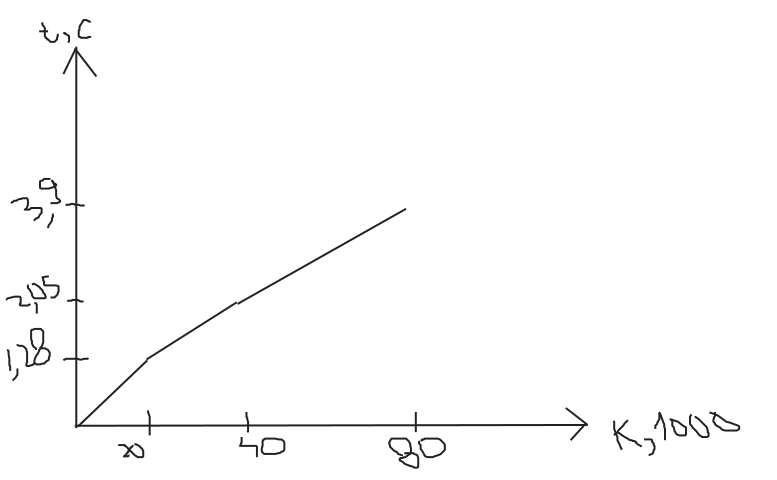
\includegraphics[scale = 0.4]{gg.png}\newline
Пояснения к графику:
\begin{enumerate}
\item За 1.28с сортируется 20000 строк
\item За 2.05с сортируется 40000 строк
\item За 3.9с сортируется 80000 строк
\end{enumerate}
Строка включается в себя ключ + значение. Исходя из графика(см. выше), можно заметить,что реализованная сортировка,является линейной.

\subsection*{Выводы}
Пожалуй, начну с оценки сложности моей сортировки. Сложность = O(k*(n + m + m + n + n)) = O(k*(3n)),k -- максимальное число разрядов, n -- количество сортируемых элементов, также при больших значениях можно пренебречь m, так как максимальное значение m = 10. С помощью поразрядной сортировки можно также сортировать различные типы данных. Например мобильные номера,автомобильные номера и тд. Также поразрядная сортировка является устойчивой, то есть сортировка, которая не меняет относительный порядок сортируемых элементов, имеющих одинаковые ключи. В ходе работы встречался с такими проблемами,как утечки памяти. Выделяя память для следующего элемента в цикле while с условием: scanf(<<\%s \%s >>, hesh->dt[i].key, hesh->dt[i].value) != EOF, случалось, что следующего элемента не было. Также какое-то время я представлял элемент hesh->dt[i]->number типом int,от чего происходил выход за пределы int и возвращались неккоректные данные. Также хотелось бы отметить, что в данной работе не использовался класс vector, так как удалось удалось реализовать необходимый тип данных с помощью структуры.

\end{document}
